% Copyright 2006 by Till Tantau
%
% This file may be distributed and/or modified
%
% 1. under the LaTeX Project Public License and/or
% 2. under the GNU Free Documentation License.
%
% See the file doc/generic/pgf/licenses/LICENSE for more details.

\section{Coordinate and Canvas Transformations}

\subsection{Overview}

\pgfname\ offers two different ways of scaling, shifting, and rotating
(these operations are generally known as \emph{transformations})
graphics: You can apply \emph{coordinate transformations} to all
coordinates and you can apply \emph{canvas transformations} to the
canvas on which you draw. (The names ``coordinate'' and ``canvas''
transformations are not standard, I introduce them only for the
purposes of this manual.)

The difference is the following:

\begin{itemize}
\item
  As the name ``coordinate transformation'' suggests, coordinate
  transformations apply only to coordinates. For example, when you
  specify a coordinate like |\pgfpoint{1cm}{2cm}| and you wish to
  ``use'' this coordinate---for example as an argument to a
  |\pgfpathmoveto| command---then the coordinate transformation matrix
  is applied to the coordinate, resulting in a new
  coordinate. Continuing the example, if the current coordinate
  transformation is ``scale by a factor of two,'' the coordinate
  |\pgfpoint{1cm}{2cm}| actually designates the point
  $(2\mathrm{cm},4\mathrm{cm})$.

  Note that coordinate transformations apply \emph{only} to
  coordinates. They do not apply to, say, line width or shadings or
  text.
\item
  The effect of a ``canvas transformation'' like ``scale by a factor
  of two'' can be imagined as follows: You first draw your picture on
  a ``rubber canvas'' normally. Then, once you are done, the whole
  canvas is transformed, in this case stretched by a factor of
  two. In the resulting image \emph{everything} will be larger: Text,
  lines, coordinates, and shadings.
\end{itemize}

In many cases, it is preferable that you use coordinate
transformations and not canvas transformations. When canvas
transformations are used, \pgfname\ looses track of the coordinates of
nodes and shapes. Also, canvas transformations often cause undesirable
effects like changing text size. For these reasons, \pgfname\ makes it
easy to setup the coordinate transformation, but a bit harder to
change the canvas transformation.


\subsection{Coordinate Transformations}

\subsubsection{How PGF Keeps Track of the Coordinate Transformation
  Matrix}

\pgfname\ has an internal coordinate transformation matrix. This
matrix is applied to coordinates ``in certain situations.'' This means
that the matrix is not always applied to every coordinate ``no matter
what.'' Rather, \pgfname\ tries to be reasonably smart at when and how
this matrix should be applied. The most prominent examples are the
path construction commands, which apply the coordinate transformation
matrix to their inputs.

The coordinate transformation matrix consists of four numbers $a$,
$b$, $c$, and $d$, and two dimensions $s$ and $t$. When the coordinate
transformation matrix is applied to a coordinate $(x,y)$ the new
coordinate $(ax+by+s,cx+dy+t)$ results. For more details on how
transformation matrices work in general, please see, for example, the
\textsc{pdf} or PostScript reference or a textbook on computer
graphics.

The coordinate transformation matrix is equal to the identity matrix
at the beginning. More precisely, $a=1$, $b=0$, $c=0$, $d=1$,
$s=0\mathrm{pt}$, and $t=0\mathrm{pt}$.

The different coordinate transformation commands will modify the
matrix by concatenating it with another transformation matrix. This
way the effect of applying several transformation commands will
\emph{accumulate}.

The coordinate transformation matrix is local to the current \TeX\
group (unlike the canvas transformation matrix, which is local to the
current |{pgfscope}|). Thus, the effect of adding a coordinate
transformation to the coordinate transformation matrix will last only
till the end of the current \TeX\ group.




\subsubsection{Commands for Relative Coordinate Transformations}

The following commands add a basic coordinate transformation to the
current coordinate transformation matrix. For all commands, the
transformation is applied \emph{in addition} to any previous
coordinate transformations.

\begin{command}{\pgftransformshift\marg{point}}
  Shifts coordinates by \meta{point}.
\begin{codeexample}[]
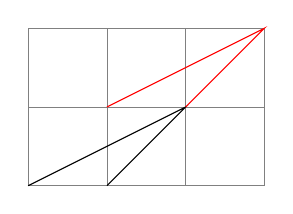
\begin{tikzpicture}
  \draw[help lines] (0,0) grid (3,2);
  \draw      (0,0) -- (2,1) -- (1,0);
  \pgftransformshift{\pgfpoint{1cm}{1cm}}
  \draw[red] (0,0) -- (2,1) -- (1,0);
\end{tikzpicture}
\end{codeexample}
\end{command}

\begin{command}{\pgftransformxshift\marg{dimensions}}
  Shifts coordinates by \meta{dimension} along the $x$-axis.
\begin{codeexample}[]
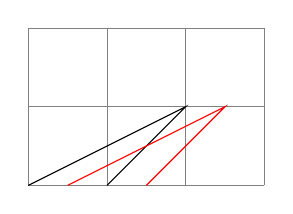
\begin{tikzpicture}
  \draw[help lines] (0,0) grid (3,2);
  \draw      (0,0) -- (2,1) -- (1,0);
  \pgftransformxshift{.5cm}
  \draw[red] (0,0) -- (2,1) -- (1,0);
\end{tikzpicture}
\end{codeexample}
\end{command}

\begin{command}{\pgftransformyshift\marg{dimensions}}
  Like |\pgftransformxshift|, only for the $y$-axis.
\end{command}

\begin{command}{\pgftransformscale\marg{factor}}
  Scales coordinates by \meta{factor}.
\begin{codeexample}[]
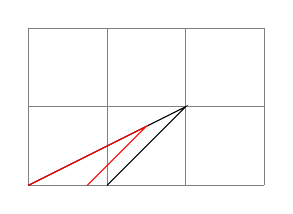
\begin{tikzpicture}
  \draw[help lines] (0,0) grid (3,2);
  \draw      (0,0) -- (2,1) -- (1,0);
  \pgftransformscale{.75}
  \draw[red] (0,0) -- (2,1) -- (1,0);
\end{tikzpicture}
\end{codeexample}
\end{command}

\begin{command}{\pgftransformxscale\marg{factor}}
  Scales coordinates by \meta{factor} in the $x$-direction.
\begin{codeexample}[]
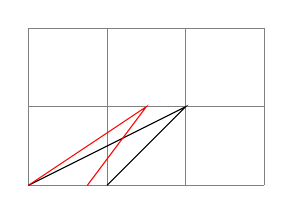
\begin{tikzpicture}
  \draw[help lines] (0,0) grid (3,2);
  \draw      (0,0) -- (2,1) -- (1,0);
  \pgftransformxscale{.75}
  \draw[red] (0,0) -- (2,1) -- (1,0);
\end{tikzpicture}
\end{codeexample}
\end{command}


\begin{command}{\pgftransformyscale\marg{factor}}
  Like |\pgftransformxscale|, only for the $y$-axis.
\end{command}


\begin{command}{\pgftransformxslant\marg{factor}}
  Slants coordinates by \meta{factor} in the $x$-direction. Here, a
  factor of |1| means $45^\circ$.
\begin{codeexample}[]
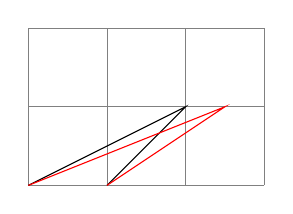
\begin{tikzpicture}
  \draw[help lines] (0,0) grid (3,2);
  \draw      (0,0) -- (2,1) -- (1,0);
  \pgftransformxslant{.5}
  \draw[red] (0,0) -- (2,1) -- (1,0);
\end{tikzpicture}
\end{codeexample}
\end{command}


\begin{command}{\pgftransformyslant\marg{factor}}
  Slants coordinates by \meta{factor} in the $y$-direction.
\begin{codeexample}[]
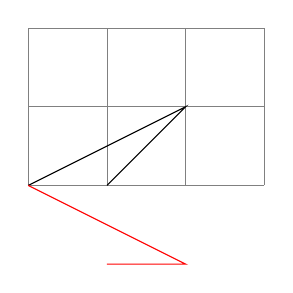
\begin{tikzpicture}
  \draw[help lines] (0,0) grid (3,2);
  \draw      (0,0) -- (2,1) -- (1,0);
  \pgftransformyslant{-1}
  \draw[red] (0,0) -- (2,1) -- (1,0);
\end{tikzpicture}
\end{codeexample}
\end{command}



\begin{command}{\pgftransformrotate\marg{degrees}}
  Rotates coordinates counterclockwise by \meta{degrees}.
\begin{codeexample}[]
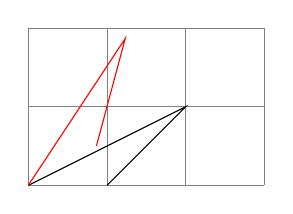
\begin{tikzpicture}
  \draw[help lines] (0,0) grid (3,2);
  \draw      (0,0) -- (2,1) -- (1,0);
  \pgftransformrotate{30}
  \draw[red] (0,0) -- (2,1) -- (1,0);
\end{tikzpicture}
\end{codeexample}
\end{command}



\begin{command}{\pgftransformtriangle\marg{a}\marg{b}\marg{c}}
  This command transforms the coordinate system in such a way that the
  triangle given by the points \meta{a}, \meta{b} and \meta{c} lies at
  the coordinates $(0,0)$, $(1\mathrm{pt},0\mathrm{pt})$ and
  $(0\mathrm{pt},1\mathrm{pt})$.
\begin{codeexample}[]
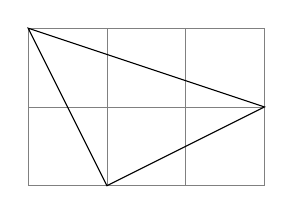
\begin{tikzpicture}
  \draw[help lines] (0,0) grid (3,2);
  \pgftransformtriangle
  {\pgfpoint{1cm}{0cm}}
  {\pgfpoint{0cm}{2cm}}
  {\pgfpoint{3cm}{1cm}}

  \draw (0,0) -- (1pt,0pt) -- (0pt,1pt) -- cycle;
\end{tikzpicture}
\end{codeexample}
\end{command}


\begin{command}{\pgftransformcm\marg{a}\marg{b}\marg{c}\marg{d}\marg{point}}
  Applies the transformation matrix given by $a$, $b$, $c$, and $d$
  and the shift \meta{point} to coordinates (in addition to any
  previous transformations already in force).
\begin{codeexample}[]
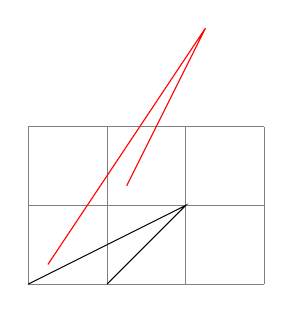
\begin{tikzpicture}
  \draw[help lines] (0,0) grid (3,2);
  \draw      (0,0) -- (2,1) -- (1,0);
  \pgftransformcm{1}{1}{0}{1}{\pgfpoint{.25cm}{.25cm}}
  \draw[red] (0,0) -- (2,1) -- (1,0);
\end{tikzpicture}
\end{codeexample}
\end{command}


\begin{command}{\pgftransformarrow\marg{start}\marg{end}}
  Shift coordinates to the end of the line going from \meta{start}
  to \meta{end} with the correct rotation.
\begin{codeexample}[]
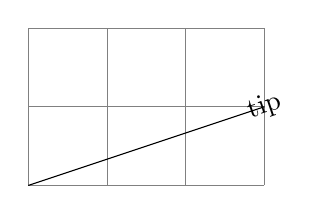
\begin{tikzpicture}
  \draw[help lines] (0,0) grid (3,2);
  \draw      (0,0) -- (3,1);
  \pgftransformarrow{\pgfpointorigin}{\pgfpoint{3cm}{1cm}}
  \pgftext{tip}
\end{tikzpicture}
\end{codeexample}
\end{command}


\begin{command}{\pgftransformlineattime\marg{time}\marg{start}\marg{end}}
  Shifts coordinates by a specific point on a line at a specific
  time. The point by which the coordinate is shifted is calculated by
  calling |\pgfpointlineattime|, see
  Section~\ref{section-pointsattime}.

  In addition to shifting the coordinate, a rotation \emph{may} also
  be applied. Whether this is the case depends on whether the \TeX\ if
  |\ifpgfslopedattime| is set to true or not.
\begin{codeexample}[]
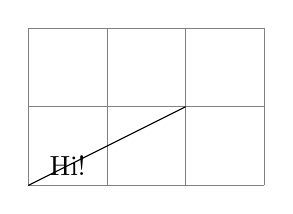
\begin{tikzpicture}
  \draw[help lines] (0,0) grid (3,2);
  \draw      (0,0) -- (2,1);
  \pgftransformlineattime{.25}{\pgfpointorigin}{\pgfpoint{2cm}{1cm}}
  \pgftext{Hi!}
\end{tikzpicture}
\end{codeexample}
\begin{codeexample}[]
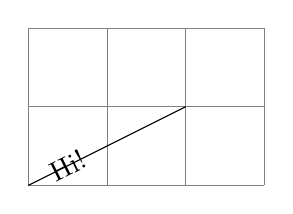
\begin{tikzpicture}
  \draw[help lines] (0,0) grid (3,2);
  \draw      (0,0) -- (2,1);
  \pgfslopedattimetrue
  \pgftransformlineattime{.25}{\pgfpointorigin}{\pgfpoint{2cm}{1cm}}
  \pgftext{Hi!}
\end{tikzpicture}
\end{codeexample}
  If |\ifpgfslopedattime| is true, another \TeX\ |\if| is important:
  |\ifpgfallowupsidedowattime|. If this is false, \pgfname\ will
  ensure that the rotation is done in such a way that text is never
  ``upside down.''

  There is another \TeX\ if that influences this command. If you set
  |\ifpgfresetnontranslationattime| to true, then, between
  shifting the coordinate and (possibly) rotating/sloping the
  coordinate, the command |\pgftransformresetnontranslations| is
  called. See the description of this command for details.
\begin{codeexample}[]
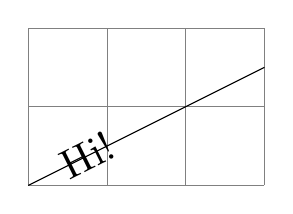
\begin{tikzpicture}
  \draw[help lines] (0,0) grid (3,2);
  \pgftransformscale{1.5}
  \draw      (0,0) -- (2,1);
  \pgfslopedattimetrue
  \pgfresetnontranslationattimefalse
  \pgftransformlineattime{.25}{\pgfpointorigin}{\pgfpoint{2cm}{1cm}}
  \pgftext{Hi!}
\end{tikzpicture}
\end{codeexample}
\begin{codeexample}[]
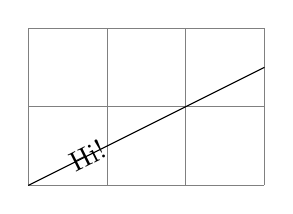
\begin{tikzpicture}
  \draw[help lines] (0,0) grid (3,2);
  \pgftransformscale{1.5}
  \draw      (0,0) -- (2,1);
  \pgfslopedattimetrue
  \pgfresetnontranslationattimetrue
  \pgftransformlineattime{.25}{\pgfpointorigin}{\pgfpoint{2cm}{1cm}}
  \pgftext{Hi!}
\end{tikzpicture}
\end{codeexample}
\end{command}


\begin{command}{\pgftransformcurveattime\marg{time}\marg{start}\marg{first
      support}\marg{second support}\marg{end}}
  Shifts coordinates by a specific point on a curve at a specific
  time, see  Section~\ref{section-pointsattime} once more.

  As for the line-at-time transformation command, |\ifpgfslopedattime|
  decides whether an additional rotation should be applied. Again, the
  value of |\ifpgfallowupsidedowattime| is also considered.
\begin{codeexample}[]
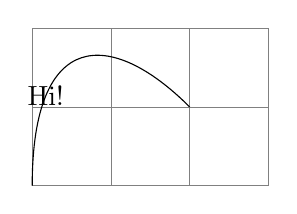
\begin{tikzpicture}
  \draw[help lines] (0,0) grid (3,2);
  \draw      (0,0) .. controls (0,2) and (1,2) .. (2,1);
  \pgftransformcurveattime{.25}{\pgfpointorigin}
    {\pgfpoint{0cm}{2cm}}{\pgfpoint{1cm}{2cm}}{\pgfpoint{2cm}{1cm}}
  \pgftext{Hi!}
\end{tikzpicture}
\end{codeexample}
\begin{codeexample}[]
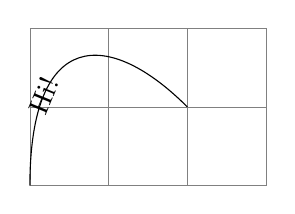
\begin{tikzpicture}
  \draw[help lines] (0,0) grid (3,2);
  \draw      (0,0) .. controls (0,2) and (1,2) .. (2,1);
  \pgfslopedattimetrue
  \pgftransformcurveattime{.25}{\pgfpointorigin}
    {\pgfpoint{0cm}{2cm}}{\pgfpoint{1cm}{2cm}}{\pgfpoint{2cm}{1cm}}
  \pgftext{Hi!}
\end{tikzpicture}
\end{codeexample}
  The value of |\ifpgfresetnontranslationsattime| is also taken into account.
\end{command}


{
  \let\ifpgfslopedattime=\relax
  \begin{textoken}{\ifpgfslopedattime}
    Decides whether the ``at time'' transformation commands also
    rotate coordinates or not.
  \end{textoken}
}
{
  \let\ifpgfallowupsidedowattime=\relax
  \begin{textoken}{\ifpgfallowupsidedowattime}
    Decides whether the ``at time'' transformation commands should
    allow the rotation be down in such a way that ``upside-down text''
    can result.
  \end{textoken}
}
{
  \let\ifpgfresetnontranslationsattime=\relax
  \begin{textoken}{\ifpgfresetnontranslationsattime}
    Decides whether the ``at time'' transformation commands should
    reset the non-translations between shifting and rotating.
  \end{textoken}
}


\subsubsection{Commands for Absolute Coordinate Transformations}

The coordinate transformation commands introduced up to now are always
applied in addition to any previous transformations. In contrast, the
commands presented in the following can be used to change the
transformation matrix ``absolutely.'' Note that this is, in general,
dangerous and will often produce unexpected effects. You should use
these commands only if you really know what you are doing.

\begin{command}{\pgftransformreset}
  Resets the coordinate transformation matrix to the identity
  matrix. Thus, once this command is given no transformations are
  applied till the end of the scope.
\begin{codeexample}[]
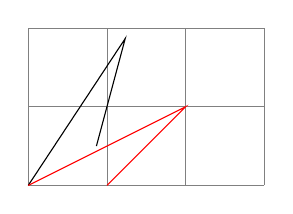
\begin{tikzpicture}
  \draw[help lines] (0,0) grid (3,2);
  \pgftransformrotate{30}
  \draw      (0,0) -- (2,1) -- (1,0);
  \pgftransformreset
  \draw[red] (0,0) -- (2,1) -- (1,0);
\end{tikzpicture}
\end{codeexample}
\end{command}


\begin{command}{\pgftransformresetnontranslations}
  This command sets the $a$, $b$, $c$, and $d$ part of the coordinate
  transformation matrix to $a=1$, $b=0$, $c=0$, and $d=1$. However,
  the current shifting of the matrix is not modified.

  The effect of this command is that any rotation/scaling/slanting is
  undone in the current \TeX\ group, but the origin is not ``moved
  back.''

  This command is mostly useful directly before a |\pgftext| command
  to ensure that the text is not scaled or rotated.
\begin{codeexample}[]
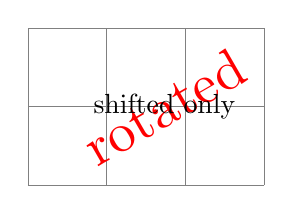
\begin{tikzpicture}
  \draw[help lines] (0,0) grid (3,2);
  \pgftransformscale{2}
  \pgftransformrotate{30}
  \pgftransformxshift{1cm}
  {\color{red}\pgftext{rotated}}
  \pgftransformresetnontranslations
  \pgftext{shifted only}
\end{tikzpicture}
\end{codeexample}
\end{command}


\begin{command}{\pgftransforminvert}
  Replaces the coordinate transformation matrix by a coordinate
  transformation matrix that ``exactly undoes the original
  transformation.'' For example, if the original transformation was
  ``scale by 2 and then shift right by 1cm'' the new one is ``shift
  left by 1cm and then scale by $1/2$.''

  This command will produce an error if the determinant of
  the matrix is too small, that is, if the matrix is near-singular.
\begin{codeexample}[]
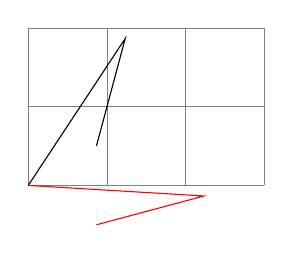
\begin{tikzpicture}
  \draw[help lines] (0,0) grid (3,2);
  \pgftransformrotate{30}
  \draw      (0,0) -- (2,1) -- (1,0);
  \pgftransforminvert
  \draw[red] (0,0) -- (2,1) -- (1,0);
\end{tikzpicture}
\end{codeexample}
\end{command}

\subsubsection{Saving and Restoring the Coordinate Transformation
  Matrix}

There are two commands for saving and restoring coordinate
transformation matrices.

\begin{command}{\pgfgettransform\marg{macro}}
  This command will (locally) define \meta{macro} to a representation
  of the current coordinate transformation matrix. This matrix can
  later on be reinstalled using |\pgfsettransform|.
\end{command}


\begin{command}{\pgfsettransform\marg{macro}}
  Reinstalls a coordinate transformation matrix that was previously
  saved using |\pgfgettransform|.
\end{command}

\begin{command}{\pgfgettransformentries\marg{macro for a}\marg{macro for b}\marg{macro for c}\marg{macro for d}\marg{macro for shift x}\marg{macro for shift y}}
	This command is similar to |\pgfgettransform| except that it stores the current coordinate transformation matrix in a set of six macros.

	The matrix can later on be reinstalled using |\pgfsettransformentries|. Furthermore, all these macros (or just a few of them) can be used as arguments for |\pgftransformcm|.
\end{command}

\begin{command}{\pgfsettransformentries\marg{a}\marg{b}\marg{c}\marg{d}\marg{shiftx}\marg{shifty}}
	Reinstalls a coordinate transformation matrix that was previously saved using the storage command |\pgfgettransformentries|. This command can also be used to replace any previously existing coordinate transformation matrix (it is thus equivalent to |\pgftransformreset| followed by |\pgftransformcm|).
\end{command}


\subsection{Canvas Transformations}

The canvas transformation matrix is not managed by \pgfname, but by
the output format like \pdf\ or PostScript. All the \pgfname\ does is
to call appropriate low-level |\pgfsys@| commands to change the canvas
transformation matrix.

Unlike coordinate transformations, canvas transformations apply to
``everything,'' including images, text, shadings, line thickness, and
so on. The idea is that a canvas transformation really stretches and
deforms the canvas after the graphic is finished.

Unlike coordinate transformations, canvas transformations are local to
the current |{pgfscope}|, not to the current \TeX\ group. This is due
to the fact that they are managed by the backend driver, not by \TeX\
or \pgfname.

Unlike the coordinate transformation matrix, it is not possible to
``reset'' the canvas transformation matrix. The only way to change it
is to concatenate it with another canvas transformation matrix or to
end the current |{pgfscope}|.

Unlike coordinate transformations, \pgfname\ does not ``keep track''
of canvas transformations. In particular, it will not be able to
correctly save the coordinates of shapes or nodes when a canvas
transformation is used.

\pgfname\ does not offer a whole set of special commands for modifying
the canvas transformation matrix. Instead, different commands allow
you to concatenate the canvas transformation matrix with a coordinate
transformation matrix (and there are numerous commands for specifying
a coordinate transformation, see the previous section).

\begin{command}{\pgflowlevelsynccm}
  This command concatenates the canvas transformation matrix with the
  current coordinate transformation matrix. Afterward, the coordinate
  transformation matrix is reset.

  The effect of this command is to ``synchronize'' the coordinate
  transformation matrix and the canvas transformation matrix. All
  transformations that were previously applied by the coordinate
  transformations matrix are now applied by the canvas transformation
  matrix.

\begin{codeexample}[]
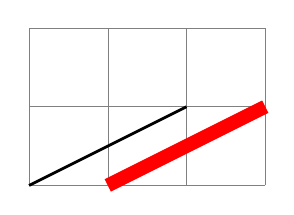
\begin{tikzpicture}
  \draw[help lines] (0,0) grid (3,2);
  \pgfsetlinewidth{1pt}
  \pgftransformscale{5}
  \draw      (0,0) -- (0.4,.2);
  \pgftransformxshift{0.2cm}
  \pgflowlevelsynccm
  \draw[red] (0,0) -- (0.4,.2);
\end{tikzpicture}
\end{codeexample}
\end{command}


\begin{command}{\pgflowlevel\marg{transformation code}}
  This command concatenates the canvas transformation matrix with the
  coordinate transformation specified by \meta{transformation code}.

\begin{codeexample}[]
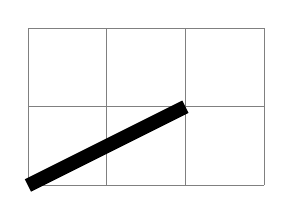
\begin{tikzpicture}
  \draw[help lines] (0,0) grid (3,2);
  \pgfsetlinewidth{1pt}
  \pgflowlevel{\pgftransformscale{5}}
  \draw      (0,0) -- (0.4,.2);
\end{tikzpicture}
\end{codeexample}
\end{command}


\begin{command}{\pgflowlevelobj\marg{transformation code}\marg{code}}
  This command creates a local |{pgfscope}|. Inside this scope,
  |\pgflowlevel| is first called with the argument
  \meta{transformation code}, then the \meta{code} is inserted.

\begin{codeexample}[]
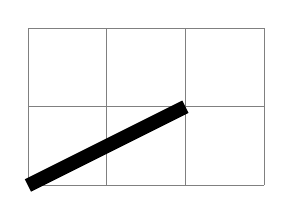
\begin{tikzpicture}
  \draw[help lines] (0,0) grid (3,2);
  \pgfsetlinewidth{1pt}
  \pgflowlevelobj{\pgftransformscale{5}}    {\draw (0,0) -- (0.4,.2);}
  \pgflowlevelobj{\pgftransformxshift{-1cm}}{\draw (0,0) -- (0.4,.2);}
\end{tikzpicture}
\end{codeexample}
\end{command}


\begin{environment}{{pgflowlevelscope}\marg{transformation code}}
  This environment first surrounds the \meta{environment contents} by
  a |{pgfscope}|. Then it calls |\pgflowlevel| with the argument
  \meta{transformation code}.

\begin{codeexample}[]
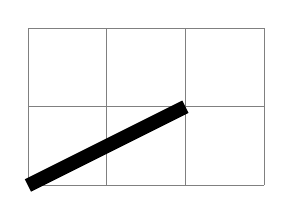
\begin{tikzpicture}
  \draw[help lines] (0,0) grid (3,2);
  \pgfsetlinewidth{1pt}
  \begin{pgflowlevelscope}{\pgftransformscale{5}}
    \draw (0,0) -- (0.4,.2);
  \end{pgflowlevelscope}
  \begin{pgflowlevelscope}{\pgftransformxshift{-1cm}}
    \draw (0,0) -- (0.4,.2);
  \end{pgflowlevelscope}
\end{tikzpicture}
\end{codeexample}
\end{environment}


\begin{plainenvironment}{{pgflowlevelscope}\marg{transformation code}}
  Plain \TeX\ version of the environment.
\end{plainenvironment}

\begin{contextenvironment}{{pgflowlevelscope}\marg{transformation code}}
  Con\TeX t version of the environment.
\end{contextenvironment}




%%% Local Variables:
%%% mode: latex
%%% TeX-master: "pgfmanual"
%%% End:
